\chapter{\LaTeX{} 畫圖}
畫圖雖然有 ipe, inkscape, gnuplot 等工具,然後使用 \verb=\includegraphics=,不
過直接在紙上畫會更精準一點,所以使用 macro 直接畫圖雖然痛苦但也精準有趣,只不
過要多記一些東西。

\section{picture}
picture 是最基本的畫圖 package,主要用 
\begin{itemize}
  \item unitlength 設定畫線單位
  \item put(x, y)\{object\} 畫預設物件,像直線,圓,方塊等等。
  \item multiput(x, y)(dx,dy)\{n\}\{object\} 畫 n 個複製物件
  \item qbezier(x1, y1)(x2, y2)(x3, y3) 貝茲曲線畫彎線,3 個控制點。
\end{itemize}
命令來畫物件,x,y 是相對於畫線單位的數字長度,multiput 的 dx, dy 是
delta 的意思,表示從 x,y 長出多少後面物件,然後複製 n 個。
預設\href{https://latexref.xyz/picture.html}{物件}有 line, circle vector ...
等等,不過有很多限制,不能隨心所欲的亂畫。
\\\\
基本設定為
\begin{verbatim}
\setlength{\unitlength}{1.2cm}
\begin{picture}(x, y)(x0, y0)
...
\end{picture}
\end{verbatim}
x,y 是畫圖方塊畫布,x0,y0 是相對於畫布的座標系統原點,這通常沒有用。例如
\begin{verbatim}
\setlength{\unitlength}{1cm}
\begin{picture}(5,5)
    \put(0,0){\line(0,1){3}}
    \put(-1,0){\line(1,1){4}}
    \put(0,2){\line(1,1){1}}
    \put(1,0){\line(1,2){2}}
\end{picture}
\end{verbatim}
上面定義了一張5x5公分的畫布,他會根據所有 input 自動調整座標系的最大最小
範圍。畫了四根線, 分別從 (0,0) (-1,0) (0,2) (1,0) 畫出,然後方向向量是根據
put 的座標的相對座標長一個長度。所以(-1,0) 開始往相對他的 (1,1),就是原本座
標的 (0,1) 方向,走 4 個 x 長度,最後就是 (-1,0) 的 x, y 各增加 (1x4, 1x4)
得 (3,4),所以 (1,0) 加上 (1x2, 2x2) 最後也到達 (3,4),不過 line 的 相對座標
只能從 -6 到 6 的整數,長度只能是正整數,要亂畫可以用 Bézier Curves 只是中間
控制點變成線性的一點,或者用 tikzpicture 比較方便。
\begin{center}
\setlength{\unitlength}{1cm}
  \begin{picture}(5,5)
    \put(0,0){\line(0,1){3}}
    \put(-1,0){\line(1,1){4}}
    \put(0,2){\line(1,1){1}}
    \put(1,0){\line(1,2){2}}
\end{picture}
\end{center}
例子就只能多看,就會了
\begin{verbatim}
\setlength{\unitlength}{1cm}
\begin{picture}(6,6)(-3,-3)
  \put(-1.5,0){\vector(1,0){3}}
  \put(2.7,-0.1){$\chi$}
  \put(0,-1.5){\vector(0,1){3}}
  \multiput(-2.5,1)(0.4,0){13} {\line(1,0){0.2}}
  \multiput(-2.5,-1)(0.4,0){13} {\line(1,0){0.2}}
  \put(0.2,1.4) {$\beta=v/c=\tanh\chi$}
  \qbezier(0,0)(0.8853,0.8853) (2,0.9640)
  \qbezier(0,0)(-0.8853,-0.8853) (-2,-0.9640)
\put(-3,-2){\circle*{0.2}}
\end{picture}
\end{verbatim}
\begin{center}
\setlength{\unitlength}{1cm}
\begin{picture}(6,6)(-3,-3)
\put(-1.5,0){\vector(1,0){3}}
\put(2.7,-0.1){$\chi$}
\put(0,-1.5){\vector(0,1){3}}
\multiput(-2.5,1)(0.4,0){13}
{\line(1,0){0.2}}
\multiput(-2.5,-1)(0.4,0){13}
{\line(1,0){0.2}}
\put(0.2,1.4)
{$\beta=v/c=\tanh\chi$}
\qbezier(0,0)(0.8853,0.8853)
(2,0.9640)
\qbezier(0,0)(-0.8853,-0.8853)
(-2,-0.9640)
\put(-3,-2){\circle*{0.2}}
\end{picture}
\end{center}
circle* 表示是個填滿黑色的實心圓。

  \subsection{Bézier Curves}
  在字型說明時,說到字型使用 Bézier Curves 來儲存字型資訊,這是由於圖形說穿
  了,不過就是每個點成線與面而已,但每個點都紀錄數值是很笨的方法,例如畫圓,
  其實只要記錄圓心與半徑,就可以了,Bézier Curves 是大多圖形軟體用來儲存曲線
  資訊的數學工具。簡單定義如下
  \\\\
  linear Bézier Curves
  \[ b(t) = (1−t)b_{0} + tb_{1} ~ for ~ t \in [0, 1] \]
  quadratic Bézier Curves
  \[ b(t) = (1−t)^{2}b_{0} + 2t(1−t)b_{1} + t^{2}b_{2} ~ for ~ t \in [0, 1]\]
  cubic Bézier Curves
  \[ b(t) = (1−t)^{3}b_{0} + 3t(1−t)^{2}b_{1} + 3t^{2}(1−t)b_{2} + t^{3}b_{3} ~ for ~ t \in [0, 1] \]
  所以一般數學式為
  \[
    b(t)
    = \sum_{i=0}^{n}
      \left( \begin{array}{c} n \\ i \end{array} \right)
      t_{i}(1 − t)^{n−i}b_{i}
      ~ for ~ t \in [0, 1]
  \]
  最基本在極端 t = 0 與 t = 1 時, 分別只有兩邊端點有效,如果是 linear ,那顯
  而易見就是一直線而已。如果是 quadratic 有以下 sampling
  \begin{center}
    \begin{tabular}{c|ccc}
      t & $(1−t)^{2}$ & $2t(1−t)$ & $t^{2}$\\
      \hline
      0 & 1 & 0 & 0 \\
      0.1 & 0.81 & 0.18 & 0.01\\
      0.2 & 0.64 & 0.32 & 0.04\\
      0.3 & 0.49 & 0.42 & 0.09\\
      0.4 & 0.36 & 0.48 & 0.16\\
      0.5 & 0.25 & 0.50 & 0.25\\
      0.6 & 0.16 & 0.48 & 0.36\\
      0.7 & 0.09 & 0.42 & 0.36\\
      0.8 & 0.04 & 0.32 & 0.64\\
      0.9 & 0.01 & 0.18 & 0.81\\
      1.0 & 0 & 0 & 1
    \end{tabular}
  \end{center}
  則會發現,$b_{1}$ 的參數值 $2t(1−t)$,從來就不會是 1,也就是這曲線到 $b_{1}$
  點前,就會轉彎向 $b_{2}$ 去, $b_{1}$ 這個點是個加權 $b_{0}$ 與 $b_{1}$ 的
  控制點,這個加權點就類似不斷的線性逼近插值 (Linear interpolation)。

  \begin{center}
    \includegraphics[width=0.6\textwidth]{images/interpolation.png}
  \end{center}

  現在 $b_{0} ~ b_{1} ~ b_{2}$ 分別是 vector,是個有 (x,y) 兩個值的參數,假
  設給與三個 (x,y) 控制點
  \begin{itemize}
    \item $b_{0} = [1,5]$
    \item $b_{1} = [3,1]$
    \item $b_{2} = [7,8]$
  \end{itemize}
  所以
  \[
    [x(b(t), y(b(t)] = (1−t)^{2} [1; 5] + 2t(1−t)[3; 1] + t^{2} [7; 8]
  \]
  而 $ x(t)= 2t^{2} + 4t + 1$ 與 $y(t) = 11t^{2} − 8t + 5$ 在 $ t \in [0,1]$ 畫
  出來得
  \begin{center}
    \begin{tabular}{c|cc}
      t & x & y\\
      \hline
      0.0 & 1.00 & 5.00 \\
      0.1 & 1.42 & 4.31 \\
      0.2 & 1.88 & 3.84 \\
      0.3 & 2.38 & 3.59 \\
      0.4 & 2.92 & 3.56 \\
      0.5 & 3.50 & 3.75 \\
      0.6 & 4.12 & 4.16 \\
      0.7 & 4.78 & 4.79 \\
      0.8 & 5.48 & 5.64 \\
      0.9 & 6.22 & 6.71 \\
      1.0 & 7.00 & 8.00
    \end{tabular}
  \end{center}
  \setlength{\unitlength}{0.5cm}
  \begin{center}
    \begin{picture}(8,8)
      \put(1,5){$b_{0}$}
      \put(3,1){$b_{1}$}
      \put(7,8){$b_{2}$}
      \put(1,5){\line(1,-2){2}}
      \qbezier(3,1)(5,4.5)(7,8)
      \qbezier(1,5)(3,1)(7,8)
    \end{picture}
    \captionof{figure}{Bézier Curves}
    \label{fig:bezier}
  \end{center}
  表示 $b_{1}$ 是兩條曲線切線的交叉點。 這其實用微分一次 $b(t)$ 也得到同樣結果
  \[
    \begin{array}{cl}
      b'(t)&=\, (2t − 2)b_{0} + (2 − 4t)b_{1} + 2tb_{2}\\
      b'(0)&=\, 2(b_{1} - b_{0})\\
      b'(1)&=\, 2(b_{2} - b_{1})\\
    \end{array}
  \]
  變化不同的控制點就會得到不同的 $x(b(t))$ 與 $y(b(t))$。
  \\\\
  在 cubic 時,控制點變成兩點,$b_{1}$ 與 $b_{2}$,變成 2 條 3 次方曲線構成完
  整曲線,$b_{0} b_{1}$ 與 $b_{2} b_{3}$ 連線也分別是切線,所以決定控制點的原
  則是找出曲線的切線上的點,一次微分切線變成
  \[
    \begin{array}{cl}
      b'(0)&=\, 3(b_{1} - b_{0})\\
      b'(1)&=\, 3(b_{3} - b_{2})\\
    \end{array}
  \]
  由於以上都是一點一點的解說,要畫出真的曲線可以用 de Casteljau's algorithm,
  能用程式就畫出平滑的曲線方法,但對很多 API 來說都是只要給控制點就可以,而
  控制點大概是那個加權在 25\% 50\% 75\% 的點,想要對控制點有感覺可以去
  % https://pomax.github.io/bezierinfo/
  \href{https://www.desmos.com/calculator/cahqdxeshd}
  {線上玩耍 Bézier Curves}。
  \\\\
  因此當 true type, otf 字型描述一個字時,是由多個 Bézier 曲線組成,當字型設
  計者拉動那些曲線與控制點時,其實後面電腦一直在計算並且轉換成螢幕上座標x,y
  的線條。

\section{pgfplots}
簡單的 pgfplots 使用 pgfplots package 跟 pgfplotsset 來設定真實大小, 是
很好畫 x-y 圖的工具。 pgfplots 是基於 tikz 的 plot 系統,能夠快速畫出座標
系統,能做 symbolic 運算畫圖, 也能引進實驗數據,畫出 X-Y 圖,等於是 \LaTeX{}
版的 gnuplot。 內定 texlive 是沒有裝,要自己 tlmgr install pgfplots,
\begin{verbatim}
\usepackage{pgfplots}
\pgfplotsset{compat=1.18,width=10cm}

  \begin{tikzpicture}

  \begin{axis}[xmin=-2,xmax=2,ymin=-2,ymax=2]
  \addplot[color=red,dashed,mark=*,samples=50]{x^2};
  \end{axis}

  \end{tikzpicture}
\end{verbatim}
\begin{center}
\begin{tikzpicture}
  \begin{axis}[xmin=-2,xmax=2,ymin=-2,ymax=2]
  \addplot[color=red,dashed,mark=*,samples=50]{x^2};
  \end{axis}
\end{tikzpicture}
\end{center}
這個例子畫了$x^2$,用了 50 個取樣點,取樣點越多就越平滑。
主要是 tikzpicture 跟 axis 這兩個 environment,然後 axis 環境的選項中括號,還
必須順序在後面, 最後要注意的是 tikzpicture 的命令是以分號 semiclone 結束
\\\\
pgfplot 還提供很方便的外部 data X-Y 圖,假設有兩個檔案 data1.txt 跟 data2.txt
\begin{verbatim}
data1.txt           data2.txt

1 10                1 30
2 20                2 70
3 40                3 100
4 80                4 170
5 160               5 280
\end{verbatim}
然後只要用 table 引進檔名,就會自己畫出 X-Y 圖
\begin{verbatim}
  \begin{tikzpicture}
    \begin{axis}[
      title={my x-y},
      xlabel={$x-axis$},
      ylabel={$y-axis$},
      legend entries={data1,data2},
      legend pos={south east}
    ]
    \addplot table {data1.txt};
    \addplot table {data2.txt};
    \end{axis}
  \end{tikzpicture}
\end{verbatim}
  \begin{center}
  \begin{tikzpicture}
    \begin{axis}[
      title={my x-y},
      xlabel={$x-axis$},
      ylabel={$y-axis$},
      legend entries={data1,data2},
      legend pos={south east}
    ]
    \addplot table {data1.txt};
    \addplot table {data2.txt};
    \end{axis}
  \end{tikzpicture}
  \end{center}
  其中還用上了 X-Y 圖的圖例標籤 legend,與X-Y軸的 label 文字。legend 的位置,
  可以從 pos 指定,south east 表示放在東南邊。
  而除了大軸用的 xlabel, ylabel 外, 座標系統的標注可以用 xticklabel,
  yticklabel 來使用
\begin{verbatim}
  \begin{tikzpicture}

  \begin{axis}[
    xmin=0,xmax=2*pi,ymin=-2,ymax=2,
    axis line=middle,
    xticklabels={$0$,$\frac{\pi}{2}$,$\pi$,$\frac{3}{2}\pi$,$2\pi$},
    xticklabel style={anchor=south west},
    xtick={0,pi/2,pi,3*pi/2,2*pi},
    xmajorgrids=true,
    grid style=dashed
  ]
  \addplot[domain=0:2*pi,color=blue]{sin(deg{x})} node[right,pos=0.3]{$f(x) = sin(x)$};

  \end{axis}

  \end{tikzpicture}
\end{verbatim}

\begin{center}
\begin{tikzpicture}

  \begin{axis}[
    xmin=0,xmax=2*pi,ymin=-2,ymax=2,
    axis lines=middle,
    xticklabels={$0$,$\frac{\pi}{2}$,$\pi$,$\frac{3}{2}\pi$,$2\pi$},
    xticklabel style={anchor=south west},
    xtick={0,pi/2,pi,3*pi/2,2*pi},
    xmajorgrids=true,
    grid style=dashed
  ]
  \addplot[domain=0:2*pi,color=blue]{sin(deg(x))} node[right,pos=0.3]{$f(x) = sin(x)$};
  \end{axis}

\end{tikzpicture}
\end{center}
使用很多選項標注文字,在 plot 裡面標注文字用 node,pos=1 表示在 sin 圖
的 100\%處標上文字,可以用 0 到 1 表示百分比。xticklabel 的 style 是標注文字
的位置,anchor 在西南,表示 xticklabel 在 x 軸的東北。

\section{TIKZ}
pgfplots 是 based 在 tikz 之上,所以他很方便,但我們也可以用 tikz 畫圖,相比較
更基本的 picture ,他有更多的選項與搭配的 library, 像樂譜,下棋,甚至還有像鴨
子, tikzducks,library 都要額外自己裝 package,但用 tlmgr 裝很快就裝起來。
\\\\
tikzpicture 比 picture 好的地方是畫 line 時,picture 需要一個整數的方向 vector
,延伸一個整數長度,因為整數參數限制,無法隨心所欲的亂畫兩個 endpoint,使用
tikzpicture 則方便多了,另外 tikzpicture 的 Bezier 曲線有 cubic,可以設定兩個
控制點。 當使用原始的 tikzpicture 時,則要用 draw 這個命令去畫圖,\LaTeX{} 畫
圖,都有個座標系統,大小會自動根據所有輸入數值,找到最大最小設定, tikz 可以
給座標名字,將來好方便使用, $x-y$ 座標多以 (x,y) 表現 ,$r-\theta$ 座標則以
($\theta$:$r$) 表示, 內定值是點, 使用內定的單位就是 pt 約等於 0.35mm ,
但也可以用 (1cm,2cm) 這種方法設定, (start-angle:end-angle:radius) 表示畫弧線,
start 跟 end angle 是從正水平 x 軸逆時針開始量測。 基本命令為
\begin{itemize}
  \item coordinate 設定不同座標點成名字,畫圖命令可以用,其實就是裡面代換。
  \item draw 一個命令給不同參數畫直線,貝茲曲線等等,但最抽象物件為 node。
  \item draw node 物件可以有 node 命令直接標注文字
\end{itemize}
\begin{verbatim}
\begin{tikzpicture}
  \coordinate (A) at (2,3);

  \draw (-2,0) -- (2,0);
  \filldraw [gray] (0,0) circle (2pt);
  \draw (-2,-2) .. controls (0,0) .. (2,-2);
  \draw (-2,2) .. controls (-1,0) and (1,0) .. (2,2);

  \draw (A) arc (30:90:2);
  \draw (A) node {在 A node 物件};
  \draw (-1,-1) node { 我是 node 物件};
  \node at (1,1) { 相對座標系 1,1 };
\end{tickpicture}
\end{verbatim}
\begin{center}
\begin{tikzpicture}
  \coordinate (A) at (2,3);
  \draw (-2,0) -- (2,0);
  \filldraw [gray] (0,0) circle (2pt);
  \draw (-2,-2) .. controls (0,0) .. (2,-2);
  \draw (-2,2) .. controls (-1,0) and (1,0) .. (2,2);
  \draw (A) arc (30:90:2);
  \draw (A) node {在 A node 物件};
  \draw (-1,-1) node { 我是 node 物件};
  \node at (1,1) { 相對座標系 1,1 };
\end{tikzpicture}
\end{center}
上面畫線用 \verb=--=  ,畫貝茲曲線用 \verb=.. controls(x,y) ..=,如果要 cubic
貝茲曲線,則多用一個 and 變成 (x1,y1) and (x2,y2), 定義一個新名字 A 等於是
(2,3) 這個點,用 node 在座標系上標上想要文字。 字串中心點才是 node 設的座標。
\\\\
例子
\begin{verbatim}
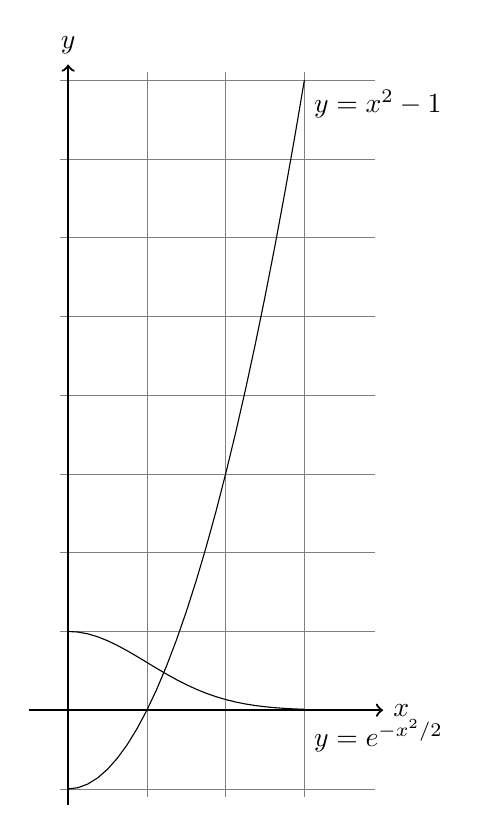
\begin{tikzpicture}
\draw[very thin,color=gray] (-0.1,-1.1) grid (3.9,8.1);
\draw[->,thick] (-0.5,0) -- (4,0) node[right] {$x$};
\draw[->,thick] (0,-1.2) -- (0,8.2) node[above] {$y$};

\draw[domain=0:3] plot (\x,{\x*\x-1}) node[below right] {$y = x^2-1$};
\draw[domain=0:3] plot (\x,{exp(-\x*\x/2)}) node[below right] {$y = e^{-x^2/2}$};
\end{tikzpicture}
\end{verbatim}

\begin{center}
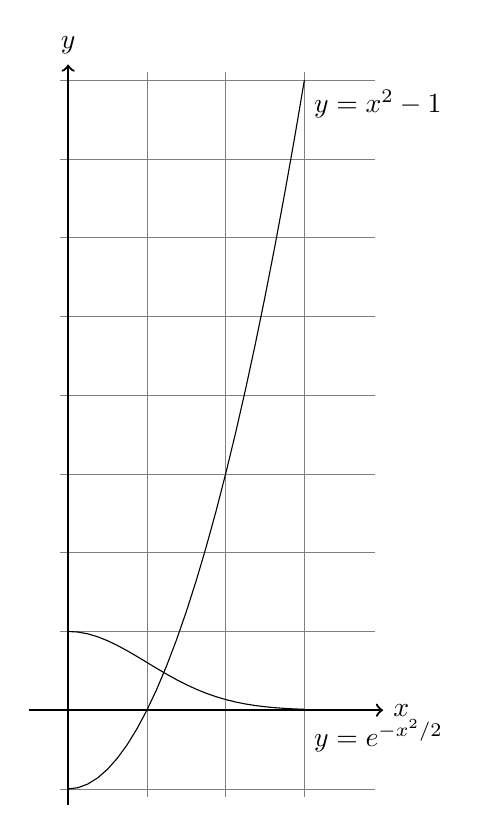
\begin{tikzpicture}
\draw[very thin,color=gray] (-0.1,-1.1) grid (3.9,8.1);
\draw[->,thick] (-0.5,0) -- (4,0) node[right] {$x$};
\draw[->,thick] (0,-1.2) -- (0,8.2) node[above] {$y$};

\draw[domain=0:3] plot (\x,{\x*\x-1}) node[below right] {$y = x^2-1$};
\draw[domain=0:3] plot (\x,{exp(-\x*\x/2)}) node[below right] {$y = e^{-x^2/2}$};
\end{tikzpicture}
\end{center}
重點是
\begin{itemize}
  \item 一樣用中括號設定參數,用 ( ) 設定起始點,終點
  \item 畫格子 grid,除了 grid 還有之前看到的 circle, rectangle...。
  \item node 寫文字, 擺設位置設定在起始點的 below, above, right, left,
    在 pgfplots 裡面用east, south, west, north 東南西北表示。
  \item 用 \verb=->= 畫箭頭
  \item 用 color 畫顏色
  \item 指定線粗細用 thin, thick ...
  \item plot 畫 symbolic 運算
  \item domain 設定 symbolic 運算範圍
\end{itemize}
顏色與粗細設定
\begin{itemize}
  \item black, red, green, blue, cyan, magenta, ...
  \item ultra thin, very thin, thin 三種 thin
  \item ultra thick, very thick, thick 三種 thick
\end{itemize}
\begin{center}
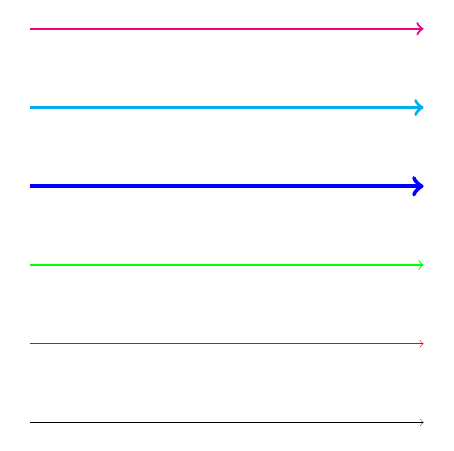
\begin{tikzpicture}
\draw[->,ultra thin, color=black] (0,1) -- (5,1);
\draw[->,very thin,color=red] (0,2) -- (5,2);
\draw[->,thin,color=green] (0,3) -- (5,3);
\draw[->,ultra thick,color=blue] (0,4) -- (5,4);
\draw[->,very thick,color=cyan] (0,5) -- (5,5);
\draw[->,thick,color=magenta] (0,6) -- (5,6);
\end{tikzpicture}
\end{center}
最後 tikzpicture 有很多 library 可以套用,只要用 usetikzlibrary 引用
,例如 patterns 跟 snakes
\begin{verbatim}
\usetikzlibrary{patterns,snakes}

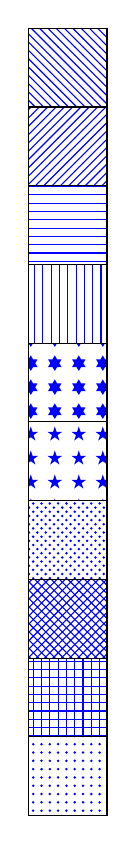
\begin{tikzpicture}
\draw[pattern=dots, pattern color=blue] (0,0) rectangle ++(1,1);
\draw[pattern=grid, pattern color=blue] (0,1) rectangle ++(1,1);
\draw[pattern=crosshatch, pattern color=blue] (0,2) rectangle ++(1,1);
\draw[pattern=crosshatch dots, pattern color=blue] (0,3) rectangle ++(1,1);
\draw[pattern=fivepointed stars, pattern color=blue] (0,4) rectangle ++(1,1);
\draw[pattern=sixpointed stars, pattern color=blue] (0,5) rectangle ++(1,1);
\draw[pattern=vertical lines, pattern color=blue] (0,6) rectangle ++(1,1);
\draw[pattern=horizontal lines, pattern color=blue] (0,7) rectangle ++(1,1);
\draw[pattern=north east lines, pattern color=blue] (0,8) rectangle ++(1,1);
\draw[pattern=north west lines, pattern color=blue] (0,9) rectangle ++(1,1);
\end{tikzpicture}
\end{verbatim}
\begin{center}
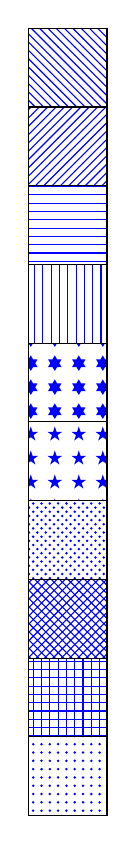
\begin{tikzpicture}
\draw[pattern=dots, pattern color=blue] (0,0) rectangle ++(1,1);
\draw[pattern=grid, pattern color=blue] (0,1) rectangle ++(1,1);
\draw[pattern=crosshatch, pattern color=blue] (0,2) rectangle ++(1,1);
\draw[pattern=crosshatch dots, pattern color=blue] (0,3) rectangle ++(1,1);
\draw[pattern=fivepointed stars, pattern color=blue] (0,4) rectangle ++(1,1);
\draw[pattern=sixpointed stars, pattern color=blue] (0,5) rectangle ++(1,1);
\draw[pattern=vertical lines, pattern color=blue] (0,6) rectangle ++(1,1);
\draw[pattern=horizontal lines, pattern color=blue] (0,7) rectangle ++(1,1);
\draw[pattern=north east lines, pattern color=blue] (0,8) rectangle ++(1,1);
\draw[pattern=north west lines, pattern color=blue] (0,9) rectangle ++(1,1);
\end{tikzpicture}
\end{center}
snakes
\begin{verbatim}
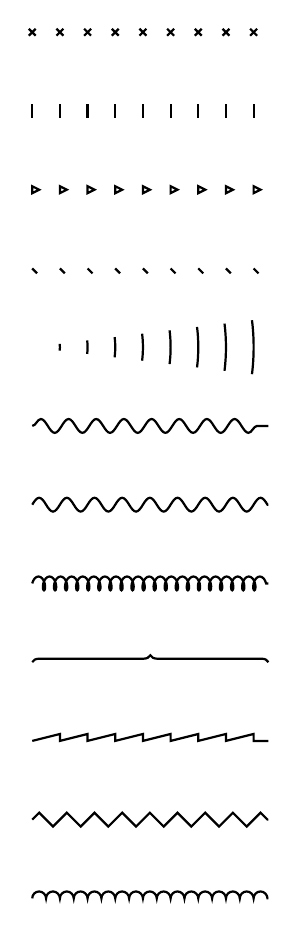
\begin{tikzpicture}[thick]
\draw[snake=bumps] (0,0) -- (3,0);
\draw[snake=zigzag] (0,1)-- (3,1);
\draw[snake=saw] (0,2) -- (3,2);
\draw[snake=brace] (0,3)-- (3,3);
\draw[snake=coil,segment length=4pt] (0,4)-- (3,4);
\draw[snake=coil,segment aspect=0] (0,5) -- (3,5);
\draw[snake=snake] (0,6) -- (3,6);
\draw[snake=expanding waves,segment angle=7] (0,7)-- (3,7);
\draw[snake=border,segment angle=-45] (0,8) -- (3,8);
\draw[snake=triangles] (0,9) -- (3,9);
\draw[snake=ticks] (0,10) -- (3,10);
\draw[snake=crosses] (0,11) -- (3,11);
\end{tikzpicture}
\end{verbatim}
\begin{center}
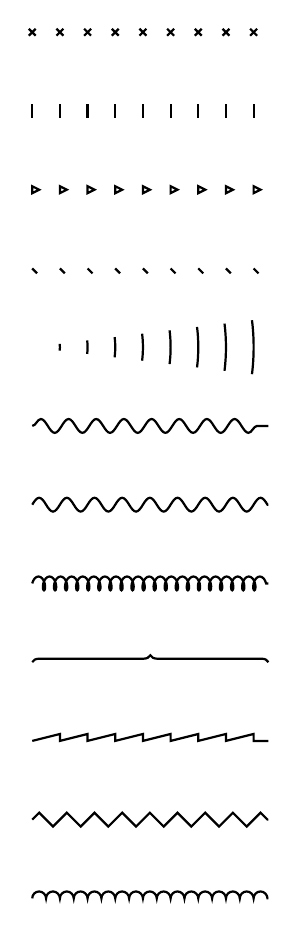
\begin{tikzpicture}[thick]
\draw[snake=bumps] (0,0) -- (3,0);
\draw[snake=zigzag] (0,1)-- (3,1);
\draw[snake=saw] (0,2) -- (3,2);
\draw[snake=brace] (0,3)-- (3,3);
\draw[snake=coil,segment length=4pt] (0,4)-- (3,4);
\draw[snake=coil,segment aspect=0] (0,5) -- (3,5);
\draw[snake=snake] (0,6) -- (3,6);
\draw[snake=expanding waves,segment angle=7] (0,7)-- (3,7);
\draw[snake=border,segment angle=-45] (0,8) -- (3,8);
\draw[snake=triangles] (0,9) -- (3,9);
\draw[snake=ticks] (0,10) -- (3,10);
\draw[snake=crosses] (0,11) -- (3,11);
\end{tikzpicture}
\end{center}
鴨子
\begin{verbatim}
\usetikzlibrary{ducks}

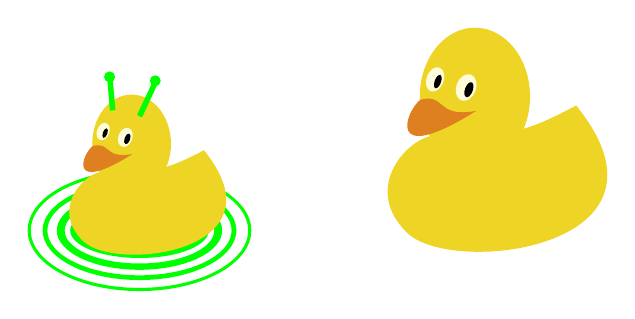
\begin{tikzpicture}
  \draw (0,0) pic[
    duck/water=green,
    duck/alien,
    ] {duck};
  \draw (4,0) pic[
    scale=1.4,
    ] {duck};
\end{tikzpicture}
\end{verbatim}
\begin{center}
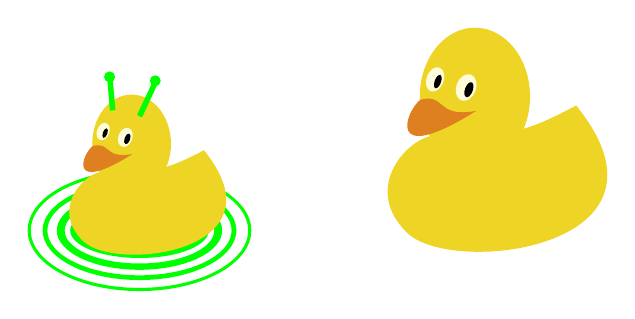
\begin{tikzpicture}
  \draw (0,0) pic[
    duck/water=green,
    duck/alien,
    ] {duck};
  \draw (4,0) pic[
    scale=1.4,
    ] {duck};
\end{tikzpicture}
\end{center}
這些工具所畫圖都能跟之前插圖用的 figure, wrapfig 共用,也能用上索引 caption。
\\\\
其實還有很多其他有趣的畫圖工具,有的畫工程圖或 x-y 圖也很漂亮,基本上三種繪圖
工具都非常多設定,所以最後還是要 google 看人家的範例改成自己想要的,無論什麼圖
,大致都能快速精準畫出。
